\documentclass[dvipsnames, tikz]{standalone}
\usepackage[bitstream-charter]{mathdesign}

\usetikzlibrary{patterns}
\definecolor{p1}{HTML}{157a6e}
\definecolor{p2}{HTML}{499f68}
\definecolor{p3}{HTML}{77b28c}
\definecolor{p4}{HTML}{CAE7D1}
\definecolor{p5}{HTML}{b4654a}
\begin{document}
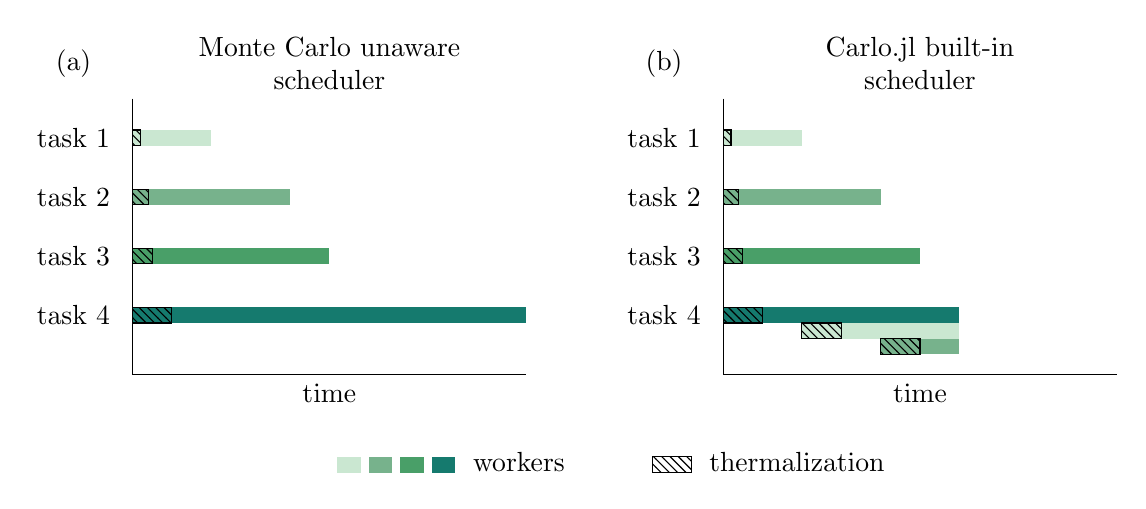
\begin{tikzpicture}[task/.style={}]
\node[task] at (-0.75, 3.25) {task 1};
\node[task] at (-0.75, 2.5) {task 2};
\node[task] at (-0.75, 1.75) {task 3};
\node[task] at (-0.75, 1.0) {task 4};
\draw[fill=p4,draw=none] (0, 3.15) rectangle ++(1, 0.2);
\draw[fill=p3,draw=none] (0, 2.40) rectangle ++(2, 0.2);
\draw[fill=p2,draw=none] (0, 1.65) rectangle ++(2.5, 0.2);
\draw[fill=p1,draw=none] (0, 0.9) rectangle ++(5, 0.2);
\draw[pattern=north west lines] (0, 3.15) rectangle ++(0.1, 0.2);
\draw[pattern=north west lines] (0, 2.40) rectangle ++(0.2, 0.2);
\draw[pattern=north west lines] (0, 1.65) rectangle ++(0.25, 0.2);
\draw[pattern=north west lines] (0, 0.9) rectangle ++(0.5, 0.2);
\draw (0,3.75) -- (0, 0.25) -- node[below]{time} (5,0.25);

\node[align=center] at (2.5, 4.2) {Monte Carlo unaware \\ scheduler};
\node at (-0.75, 4.2) {(a)};

\begin{scope}[shift={(7.5,0)}]
\node[task] at (-0.75, 3.25) {task 1};
\node[task] at (-0.75, 2.5) {task 2};
\node[task] at (-0.75, 1.75) {task 3};
\node[task] at (-0.75, 1.0) {task 4};
\draw[fill=p4,draw=none] (0, 3.15) rectangle ++(1, 0.2);
\draw[fill=p3,draw=none] (0, 2.40) rectangle ++(2, 0.2);
\draw[fill=p2,draw=none] (0, 1.65) rectangle ++(2.5, 0.2);
\draw[fill=p1,draw=none] (0, 0.9) rectangle ++(3, 0.2);
\draw[pattern=north west lines] (0, 3.15) rectangle ++(0.1, 0.2);
\draw[pattern=north west lines] (0, 2.40) rectangle ++(0.2, 0.2);
\draw[pattern=north west lines] (0, 1.65) rectangle ++(0.25, 0.2);
\draw[pattern=north west lines] (0, 0.9) rectangle ++(0.5, 0.2);

\draw[fill=p4,draw=none] (1, 0.7) rectangle ++(2, 0.2);
\draw[pattern=north west lines] (1, 0.7) rectangle ++(0.5, 0.2);
\draw[fill=p3,draw=none] (2, 0.5) rectangle ++(1, 0.2);
\draw[pattern=north west lines] (2, 0.5) rectangle ++(0.5, 0.2);
\draw (0,3.75) -- (0, 0.25) -- node[below]{time} (5,0.25);
\node[align=center] at (2.5, 4.2) {Carlo.jl built-in\\scheduler};
\node at (-0.75, 4.2) {(b)};
\end{scope}
\begin{scope}[shift={(4.6,-1)}]
\draw[fill=p4, draw=none] (-2,0) rectangle ++ (0.3, 0.2);
\draw[fill=p3, draw=none] (-1.6,0) rectangle ++ (0.3, 0.2);
\draw[fill=p2, draw=none] (-1.2,0) rectangle ++ (0.3, 0.2);
\draw[fill=p1, draw=none] (-0.8,0) rectangle ++ (0.3, 0.2);
\node[anchor=west] at (-0.4, 0.13) {workers};
\draw[pattern=north west lines] (2,0) rectangle ++ (0.5, 0.2);
\node[anchor=west] at ( 2.6, 0.13) {thermalization};
\end{scope}
\end{tikzpicture}
\end{document}
